\documentclass{standalone}
\usepackage{tikz}
\usepackage{tikz-feynman} % Paquete para diagramas de Feynman
\begin{document}

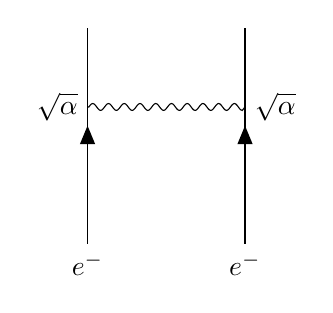
\begin{tikzpicture}
    \begin{feynman}
        % Nodos de partículas
        \vertex (i1) at (-1,-1) {$e^-$};
        \vertex (f1) at (-1,2);
        \vertex [dot, label=left:$\sqrt{\alpha}$] (v1) at (-1,1); % Etiqueta en v1
        \vertex [dot, label=right:$\sqrt{\alpha}$] (v2) at (1,1); % Etiqueta en v2
        \vertex (i2) at (1,-1) {$e^-$};
        \vertex (f2) at (1,2);
        
        % Diagramas de líneas
        \diagram* {
            (i1) --[fermion] (f1), % Línea del primer electrón
            (i2) --[fermion] (f2), % Línea del segundo electrón
            (v1) --[photon] (v2),  % Línea del fotón virtual
        };
    \end{feynman}
\end{tikzpicture}

\end{document}
